\documentclass[tikz,border=3pt]{standalone}
\usepackage{amsmath,amssymb}
\usepackage{xcolor}
\usepackage{tikz}
\usetikzlibrary{arrows.meta,backgrounds,positioning}

\definecolor{inputfill}{HTML}{BFE3C0}
\definecolor{inputdraw}{HTML}{24592B}
\definecolor{outputfill}{HTML}{F1BBB5}
\definecolor{outputdraw}{HTML}{72231F}
\definecolor{edgecolor}{HTML}{2B4472}
\definecolor{textcolor}{HTML}{172033}

\tikzset{
  >=Latex,
  input neuron/.style={
    circle,
    draw=inputdraw,
    fill=inputfill,
    line width=0.85pt,
    minimum size=10mm,
    inner sep=0pt,
    font=\bfseries\boldmath\normalsize
  },
  hidden neuron/.style={
    circle,
    draw=edgecolor,
    fill=hiddenfill,
    line width=0.9pt,
    minimum size=10mm,
    inner sep=0pt,
    font=\bfseries\boldmath\normalsize
  },
  output neuron/.style={
    circle,
    draw=outputdraw,
    fill=outputfill,
    line width=0.85pt,
    minimum size=10mm,
    inner sep=0pt,
    font=\bfseries\boldmath\normalsize
  },
  connection/.style={
    draw=edgecolor!48,
    line width=0.50pt,
    -{Latex[length=1.8mm,width=1.25mm]}
  },
  layer title/.style={
    font=\bfseries\boldmath\small,
    text=textcolor,
    align=center
  },
  parameter/.style={
    font=\bfseries\small,
    text=textcolor,
    align=center
  }
}

\definecolor{hiddenfill}{HTML}{CBC9F2}

\newcommand{\connectinputhidden}[2]{%
  \begin{scope}[on background layer]
    \foreach \i in {#1}{
      \foreach \h in {#2}{
        \draw[connection] (I-\i) -- (H-\h);
      }
    }
  \end{scope}
}

\newcommand{\connecthiddenoutput}[2]{%
  \begin{scope}[on background layer]
    \foreach \h in {#1}{
      \foreach \j in {#2}{
        \draw[connection] (H-\h) -- (O-\j);
      }
    }
  \end{scope}
}


\begin{document}
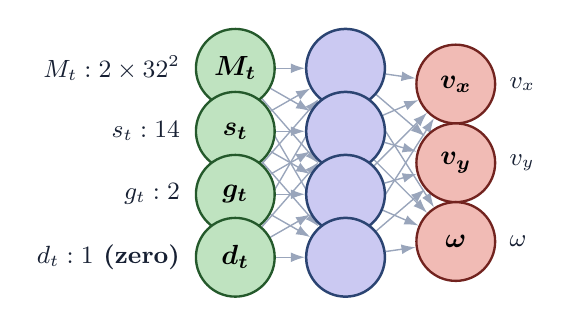
\begin{tikzpicture}[x=1cm,y=1cm]
  \node[input neuron] (I-1) at (0.00,3.25) {$M_t$};
  \node[input neuron] (I-2) at (0.00,2.45) {$s_t$};
  \node[input neuron] (I-3) at (0.00,1.65) {$g_t$};
  \node[input neuron] (I-4) at (0.00,0.85) {$d_t$};

  \node[hidden neuron] (H-1) at (1.40,3.25) {};
  \node[hidden neuron] (H-2) at (1.40,2.45) {};
  \node[hidden neuron] (H-3) at (1.40,1.65) {};
  \node[hidden neuron] (H-4) at (1.40,0.85) {};

  \node[output neuron] (O-1) at (2.80,3.05) {$v_x$};
  \node[output neuron] (O-2) at (2.80,2.05) {$v_y$};
  \node[output neuron] (O-3) at (2.80,1.05) {$\omega$};

  \connectinputhidden{1,2,3,4}{1,2,3,4}
  \connecthiddenoutput{1,2,3,4}{1,2,3}

  \node[parameter,anchor=east] at (-0.58,3.25) {$M_t:2\times32^2$};
  \node[parameter,anchor=east] at (-0.58,2.45) {$s_t:14$};
  \node[parameter,anchor=east] at (-0.58,1.65) {$g_t:2$};
  \node[parameter,anchor=east] at (-0.58,0.85) {$d_t:1$ (zero)};
  \node[parameter,anchor=west] at (3.36,3.05) {$v_x$};
  \node[parameter,anchor=west] at (3.36,2.05) {$v_y$};
  \node[parameter,anchor=west] at (3.36,1.05) {$\omega$};
\end{tikzpicture}
\end{document}
